\documentclass[10pt]{article}

\usepackage[T2A]{fontenc}
\usepackage[utf8x]{inputenc}

\usepackage[english,russian]{babel}
\usepackage{graphics, graphicx}

\usepackage{amsmath}
\usepackage{amssymb}
\usepackage{amsfonts}


\usepackage[left=20mm, top=20mm, right=20mm, bottom=20mm, nohead, nofoot, footskip=15pt]{geometry}

\usepackage{color}
\usepackage{epsfig}
\usepackage{bm}
\usepackage[colorlinks,urlcolor=blue]{hyperref}
\usepackage{tikz}
\usepackage{pgfplots}



\tolerance=1
\emergencystretch=\maxdimen
\hyphenpenalty=10000
\hbadness=10000


\author{Дмитриев Леонид}

\title{Отчет по первой лабораторной работе по сегментации изображений}

\begin{document}
	{
		\LARGE
		\maketitle
	}
	
	\clearpage
	
	
	{ \large \tableofcontents} 
	
	\clearpage
	
	
	
	\section*{Постановка задачи}
	\addcontentsline{toc}{section}{Постановка задачи}
	
	Задача заключается в разработке и реализации программы для работы с изображениями фишек Тантрикс, обеспечивающей функционал, требуемый для класса сложности Intermediate:
	
	\begin{enumerate}
		\item Определение типа фишки по входному изображению, содержащему одну фишку.
		
		\item Определение типа и расположения всех фишек, находящихся во входном избражении.
	\end{enumerate}
	
	
	\section*{Описание данных}
	\addcontentsline{toc}{section}{Описание данных}
	
	Игровой набор Тантрикс состоит из 10 фишек, представленных на рисунке (файл Dozen\_0.bmp).
	
	
	\begin{figure}[h]
		\begin{center}
			{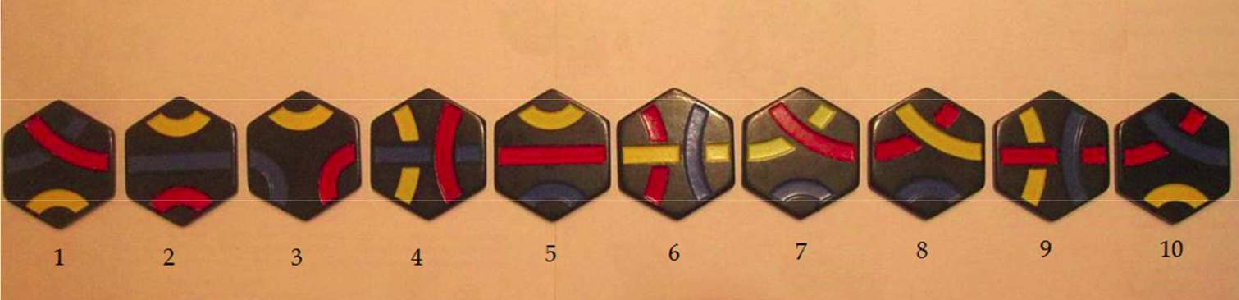
\includegraphics[width=1.0\linewidth]{data/Dozen_0.pdf}}
		\end{center}
	    \caption{Пример с правильной классификацией всех 10 типов имеющихся фишек.}
		\label{ris:image1}
	\end{figure}
	
	
	Каждая фишка представляет собой правильный шестиугольник черного цвета, на котором изображены сегменты трёх линий синего, красного и жёлтого цветов.
	
	В простых случаях на картинках изображена одна фишка, а в более сложных несколько.
	
	
	\begin{figure}[h]
		\begin{minipage}[h]{0.3\linewidth}
			\begin{center}
				{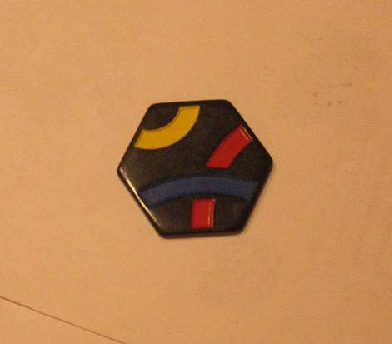
\includegraphics[width=1.0\linewidth]{data/Single_1-1.pdf}}
			\end{center}
		\end{minipage}
		\hfill
		\begin{minipage}[h]{0.3\linewidth}
			\begin{center}
				{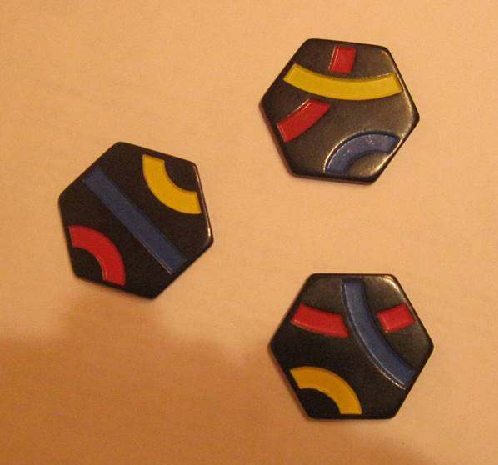
\includegraphics[width=1.0\linewidth]{data/Group_1-1.pdf}}
			\end{center}
		\end{minipage}
		\hfill
		\begin{minipage}[h]{0.3\linewidth}
			\begin{center}
				{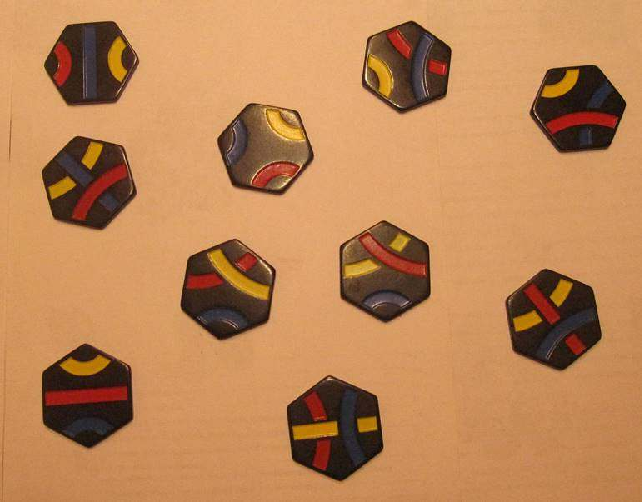
\includegraphics[width=1.0\linewidth]{data/Group_5.pdf}}
			\end{center}
		\end{minipage}
		\caption{Примеры входных изображений: для задачи 1 (слева) и для задачи 2 (в центре и справа).}
		\label{ris:image2}
	\end{figure}
	
	
	\section*{Описание метода решения}
	\addcontentsline{toc}{section}{Описание метода решения}
	
	В первую очередь было замечено, что решение задачи опредления типа одной единственной фишки в кадре вкладывается в решение задачи опредления типа и местоположения всех фишек на кадре. Поэтому далее решалась только более общая задача.
	
	Далее описаны основные моменты влгоритма, решающего поставленную задачу.
	
	
	\subsection*{Преобразования изображения для поиска контуров}
	\addcontentsline{toc}{subsection}{Преобразования изображения}
	
	Для опредлениия контуров необходимо подсветить темные объекты на изображении, а фон обнулить. Сначала картинка преобразовывается в черно-белый спектр. Далее используется гауссов фильтр для сглаживания изображения. А затем применяется инвертированная бинаризация (так чтобы темная поверхность фишек стала максимально яркой, а все остальное черным).
	
	Для определения типа фишки необходима информация о цветных контурах внутри него. Сначала картинка преобразовывается в тип HSV, а затем по опредленному диапазону тона, насыщенности, значений находится маска нужных цветов (диапазон определен экспериментально).
	
	В итоге к построенным маскам применяется функция поиска контуров из библиотеки opencv, с помощью которой для каждого шестиугольника и цветного элемента внутри фишек находится обход точек по границе.
	
	\begin{figure}[h]
		\begin{minipage}[h]{0.19\linewidth}
			\begin{center}
				{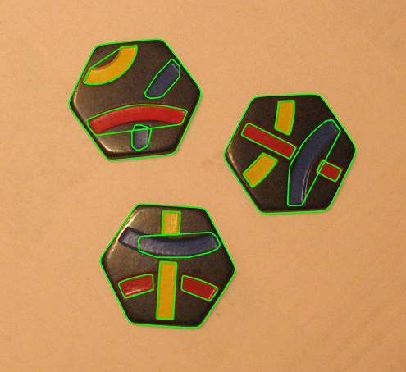
\includegraphics[width=1.0\linewidth]{data/contour_exampler.pdf}}
			\end{center}
		\end{minipage}
		\hfill
		\begin{minipage}[h]{0.19\linewidth}
			\begin{center}
				{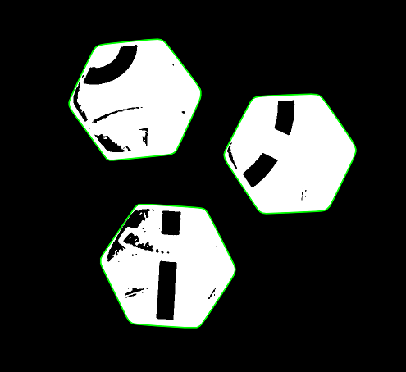
\includegraphics[width=1.0\linewidth]{data/hex_example.pdf}}
			\end{center}
		\end{minipage}
		\hfill
		\begin{minipage}[h]{0.19\linewidth}
			\begin{center}
				{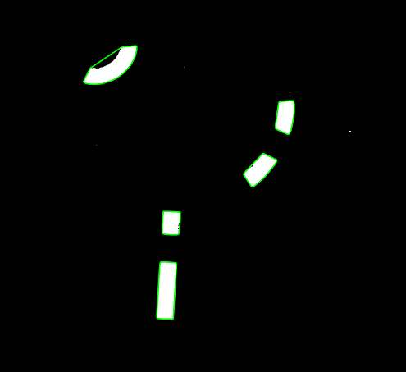
\includegraphics[width=1.0\linewidth]{data/yellow_example.pdf}}
			\end{center}
		\end{minipage}
	    \hfill
	    \begin{minipage}[h]{0.19\linewidth}
	    	\begin{center}
	    		{
\includegraphics[width=1.0\linewidth]{data/blue_example.pdf}}
	    	\end{center}
	    \end{minipage}
        \hfill
        \begin{minipage}[h]{0.19\linewidth}
        	\begin{center}
        		{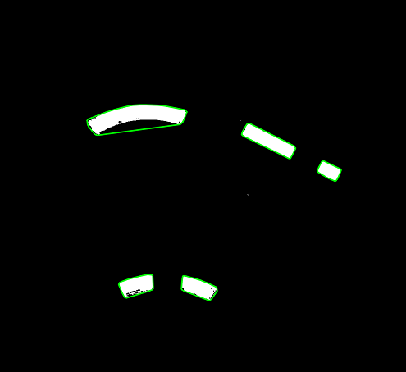
\includegraphics[width=1.0\linewidth]{data/red_example.pdf}}
        	\end{center}
        \end{minipage}
	    
		\caption{Примеры определения контуров на преобразованном изображении.}
		\label{ris:image3}
	\end{figure}
	
	После поиска контуров могли возникнуть шумовые контуры как фишек, так и цветных компонент. Они удаляются по разным правилам, например: по площади относительно остальных фигур или по расположению внутри других фигур.
	
	
	\subsection*{Построение признаковых описаний по контурам фишек}
	\addcontentsline{toc}{subsection}{Построение признаковых описаний по контурам фишек}
	
	Полученные конутры необходимо преобразовать в удобный для анализа вид.
	
	В случае правильного шестиугольника полезно найти 6 угловых точек. Для этого сначала удаляются точки образующие с соседними угол, близкий к 180 градусам. После этого остаются только точки находящиеся близко к углам. Для них применяется алгоритм кластеризации с 6 кластерами, центроиды которого и являются приближенными угловыми точками.
	
	Контуры цветных компонент для упрощения покрываются минимальными прямоугольниками.
	
	\begin{figure}[h]
		\begin{minipage}[h]{0.22\linewidth}
			\begin{center}
				{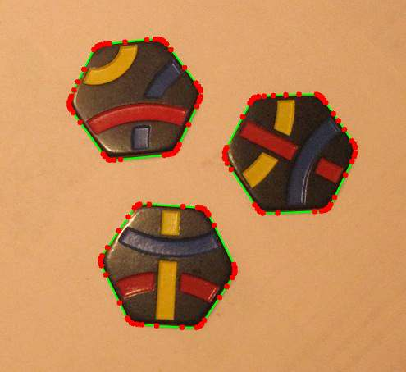
\includegraphics[width=1.0\linewidth]{data/contour_points_example.pdf}}
			\end{center}
		\end{minipage}
		\hfill
		\begin{minipage}[h]{0.22\linewidth}
			\begin{center}
				{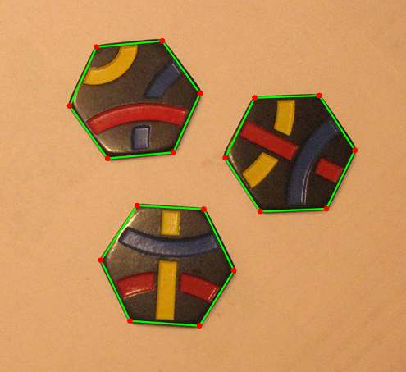
\includegraphics[width=1.0\linewidth]{data/hex_points_example.pdf}}
			\end{center}
		\end{minipage}
		\hfill
		\begin{minipage}[h]{0.22\linewidth}
			\begin{center}
				{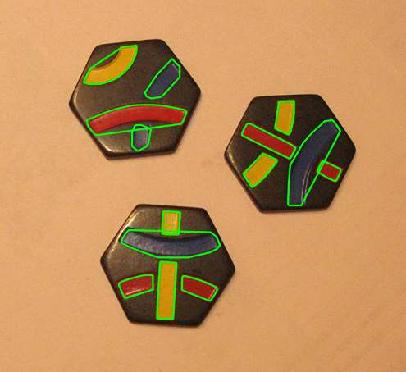
\includegraphics[width=1.0\linewidth]{data/cont_col_example.pdf}}
			\end{center}
		\end{minipage}
		\hfill
		\begin{minipage}[h]{0.22\linewidth}
			\begin{center}
				{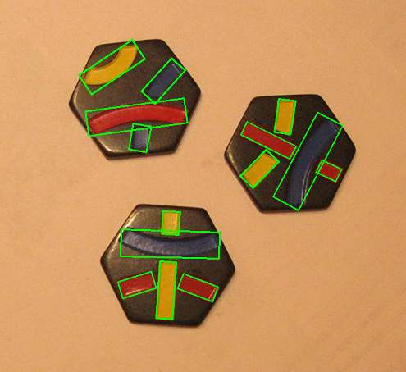
\includegraphics[width=1.0\linewidth]{data/rect_example.pdf}}
			\end{center}
		\end{minipage}
		
		\caption{Примеры определения контуров на преобразованном изображении.}
		\label{ris:image4}
	\end{figure}
	
	Можно заметить, что каждая цветная компонента соединена ровно с двумя ребрами шестиугольника (причем эти ребра принадлежат только этой компоненте). Также каждая компонента либо один раз пересечена другой компонентой, либо цела.
	
	Зная для каждого цвета соответствующие ему стороны шестиугольника и факт пересеченности можно однозначно определить тип фишки.
	
	Далее можно заметить, что центры меньших сторон прямоугольников соотв. цветным компонентам ближе всего к нужному центру сторон шестиугольника. А факт пересеченности определяется по кол-ву связных компонент данного цвета.
	
	По данным признакам строится исчерпывающее описание наблюдаемой фишки.
	
	Но в связи с различными ошибками на любом из этапов данное описание может оказаться неполным или некорректным. Одним из способов привнесения большей стабильности служит алгоритм восстановления одного из цветов по двум другим (при условии, что они определены корректно).
	
	Очевидно, что при опредлении сторон шестиугольника для двух цветов и факта пересеченности этих двух цветов, третьему цвету останется только одно возможное состояние.
	
	
	\subsection*{Определение типа фишки по признаковому описанию}
	\addcontentsline{toc}{subsection}{Определение типа фишки по признаковому описанию}
	
	Имея описание фишки, полученное на предыдущем шаге, можно лекго установить тип фишки, если заранее описать все имеющиеся типы в таком же формате и просто сравнить с каждым из них.
	
	
	\section*{Описание программной реализации}
	\addcontentsline{toc}{section}{Описание программной реализации}
	
	Для запуска пргораммы решения:
	\begin{enumerate}
		\item python main.py {-}{-}mode single {-}{-}files <filepath>
		
		Программа прочтет картинку из <filepath> и напечатает номер типа фишки и его представление в указанном выше формате.
		
		\item python main.py {-}{-}mode group {-}{-}files <src\_filepath> <dest\_filepath> [{-}{-}show False]
		
		Программа прочтет картинку из <src\_filepath> и запишет картинку такого же размера в <dest\_filepath>. В результирующей картинке поверх каждой опредленной фишки будет написан ее тип.
		Так же опционально возможно указать, выводить ли окно с результатом. 
	\end{enumerate}
	
	
	\section*{Эксперименты}
	\addcontentsline{toc}{section}{Эксперименты}
	
	
	\begin{figure}[h]
		{
		\begin{minipage}[h]{0.47\linewidth}
			\begin{center}
				{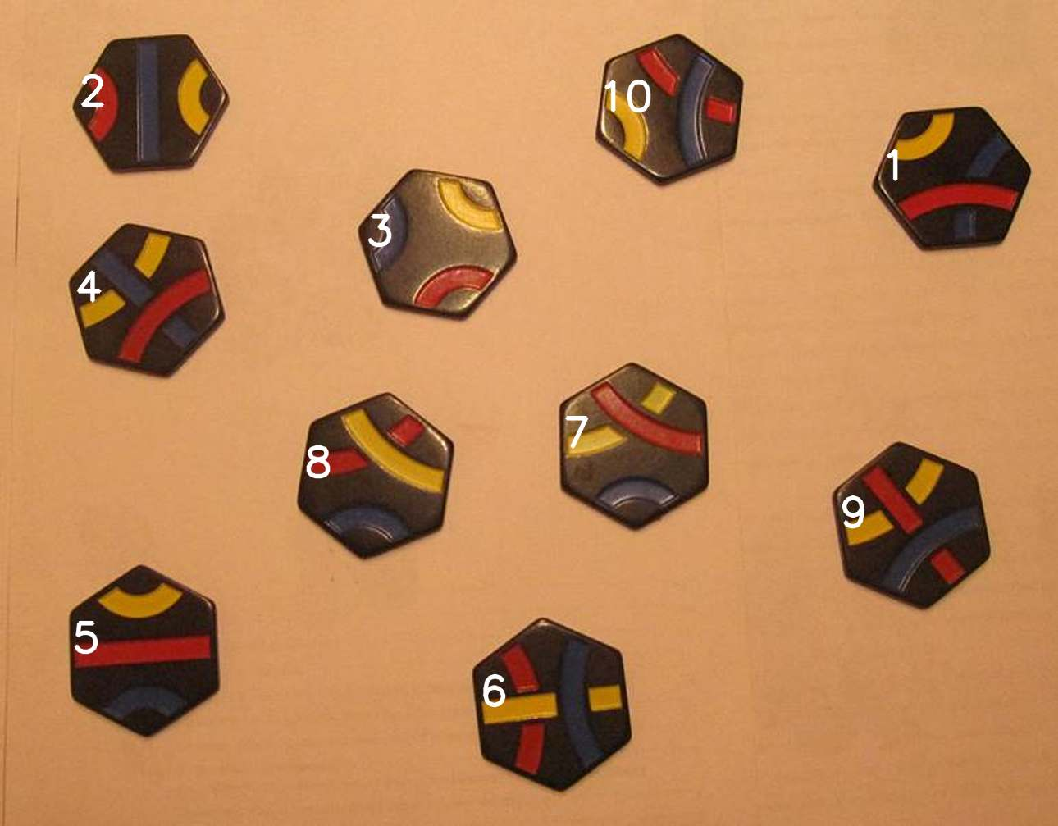
\includegraphics[width=1.0\linewidth]{data/result-3.pdf}}
			\end{center}
		\end{minipage}
	    \hfill
	    \begin{minipage}[h]{0.4\linewidth}
	    	\begin{center}
	    		{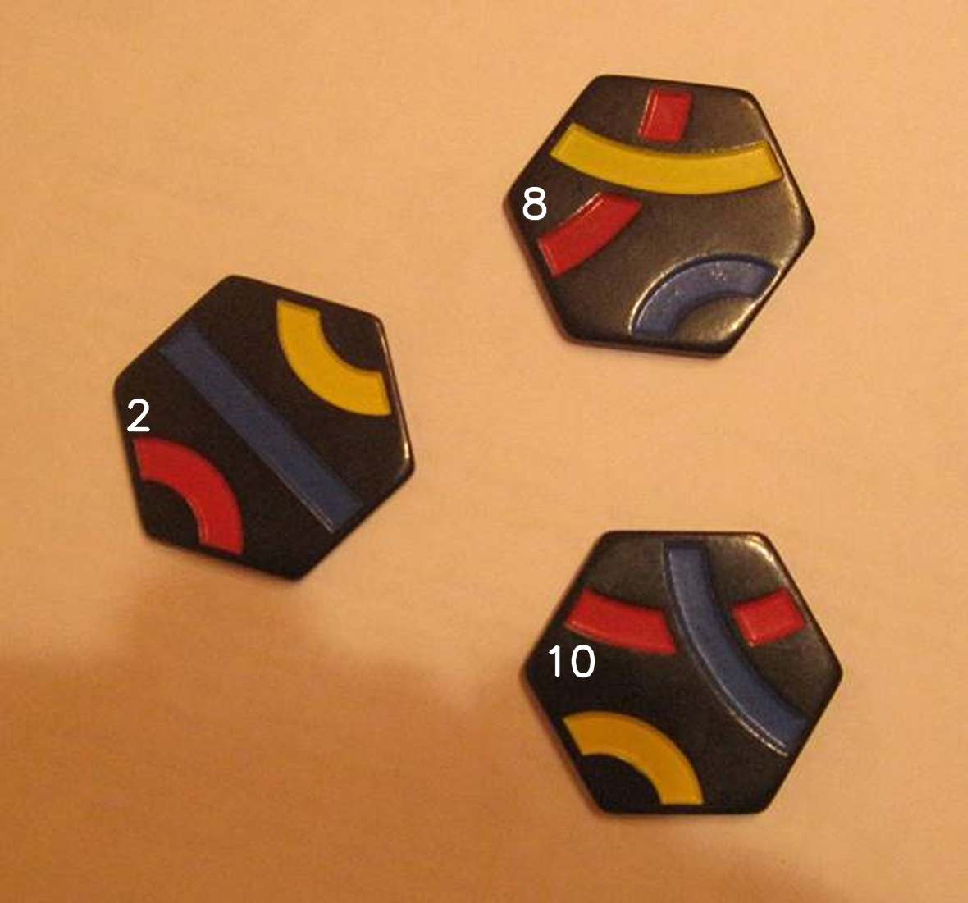
\includegraphics[width=1.0\linewidth]{data/result-4.pdf}}
	    	\end{center}
	    \end{minipage}
	    }
        \vfill
		
		\begin{minipage}[h]{\linewidth}
			\begin{center}
				{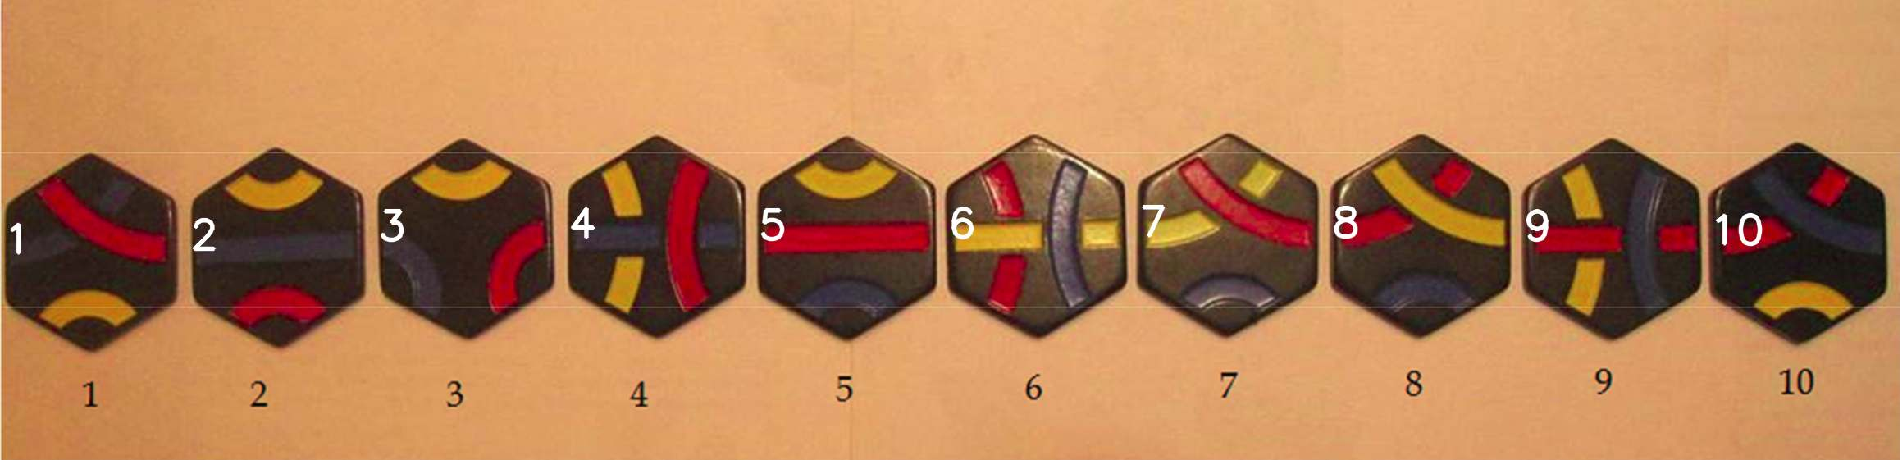
\includegraphics[width=1.0\linewidth]{data/result-5.pdf}}
			\end{center}
		\end{minipage}
	
		
		\caption{Примеры результатов программы.}
		\label{ris:image5}
	\end{figure}
	
	
	
	\section*{Выводы}
	\addcontentsline{toc}{section}{Выводы}
	
	Была решена задача распознования фишек формы праавильного шестиугольника с расположенными на нем линиями разных цветов и реализована соответствующая программа.
	
	
\end{document}
